\documentclass{article}

\usepackage{fontspec}
\usepackage{fullpage}
\usepackage{multicol}
\usepackage{multirow}
\usepackage{tikz}

\begin{document}

\newfontfamily\swfill{SuttonSignWritingFill.ttf}
\newfontfamily\swline{SuttonSignWritingLine.ttf}
\newcommand{\bul}{\hfil$\bullet$&}
\renewenvironment{glossary}{\begin{multicols}{5}\begin{center}}{\end{center}\end{multicols}}
\setcounter{secnumdepth}{0}
\setlength{\columnseprule}{1pt}

\section{Supplement For Lesson 13}

\begin{center}
\it
Objectives inspired by, vocabulary transcribed from, and sentences and story by Bill Vicars.

Handshape photos by Adam Frost.

No endorsement implied nor given by either.
\end{center}

\subsection{Objectives}

\begin{tabular}{p{1cm}p{14cm}}
\bul I have completed the objectives for this lesson.\\
\bul I know which base symbols are in Symbol Groups lip and mouth.\\
\bul I am able to read, write, and sign half of the ASL handshapes in symbol group nine.\\
\bul I am able to recognize the vocabulary for this lesson.\\
\bul I am able to read the practice sentences for this lesson.\\
\bul I am able to read the practice story for this lesson.\\
\end{tabular}

\subsection{Symbol Groups Lip and Mouth}

The twenty-fifth Symbol Group we informally call lip, though it's official name is ``Mouth Lips''.

\begin{center}
\begin{tabular}{rcrc}
\textbf{Base Symbol}&\textbf{Example}&\textbf{Base Symbol}&\textbf{Example}\\
Mouth Closed Neutral         &B518x518S33b00482x483&Mouth Closed Forward     &B518x518S33c00482x483\\
Mouth Closed Contact         &B518x518S33d00482x483&Mouth Smile              &B518x518S33e00482x483\\
Mouth Smile Wrinkled         &B518x518S33f00482x483&Mouth Smile Open         &B518x518S34000482x483\\
Mouth Frown                  &B518x518S34100482x483&Mouth Frown Wrinkled     &B518x518S34200482x483\\
Mouth Frown Open             &B518x518S34300482x483&Mouth Open Circle        &B518x518S34400482x483\\
Mouth Open Forward           &B518x518S34500482x483&Mouth Open Wrinkled      &B518x518S34600482x483\\
Mouth Open Oval              &B518x518S34700482x483&Mouth Open Oval Wrinkled &B518x518S34800482x483\\
Mouth Open Oval Yawn         &B518x518S34900482x483&Mouth Open Rectangle     &B518x518S34a00482x483\\
Mouth Open Rectangle Wrinkled&B518x518S34b00482x483&Mouth Open Rectangle Yawn&B518x518S34c00482x483\\
Mouth Kiss                   &B518x518S34d00482x483&Mouth Kiss Forward       &B518x518S34e00482x483\\
Mouth Kiss Wrinkled          &B518x518S34f00482x483&Mouth Tense              &B518x518S35000482x483\\
Mouth Tense Forward          &B518x518S35100482x483&Mouth Tense Sucked       &B518x518S35200482x483\\
Lips Pressed Together        &B518x518S35300482x483&Lip Lower Over Upper     &B518x518S35400482x483\\
Lip Upper Over Lower         &B518x518S35500482x483&Mouth Corners            &B518x518S35600482x483\\
Mouth Wrinkles Single        &B518x518S35700482x483&Mouth Wrinkles Double    &B518x518S35800482x483\\
\end{tabular}
\end{center}

The twenty-sixth Symbol Group we informally call mouth, though it's official name is ``Tongue Teeth Chin Neck''.

\begin{center}
\begin{tabular}{rcrc}
\textbf{Base Symbol}&\textbf{Example}&\textbf{Base Symbol}&\textbf{Example}\\
Tongue Sticks Out Far      &B518x518S35900482x483&Tongue Licks Lips              &B518x518S35a00482x483\\
Tongue Tip Between Lips    &B518x518S35b00482x483&Tongue Tip Touches Inside Mouth&B518x518S35c00482x483\\
Tongue Inside Mouth Relaxed&B518x518S35d00482x483&Tongue Moves Against Cheek     &B520x518S35e00481x483\\
Tongue Center Sticks Out   &B518x518S35f00482x483&Tongue Center Inside Mouth     &B518x518S36000482x483\\
Teeth                      &B518x518S36100482x483&Teeth Movement                 &B518x518S36200482x483\\
Teeth on Tongue            &B518x518S36300482x483&Teeth on Tongue Movement       &B518x518S36400482x483\\
Teeth on Lips              &B518x518S36500482x483&Teeth on Lips Movement         &B518x518S36600482x483\\
Teeth Bite Lips            &B518x518S36700482x483&Jaw Movement Wall Plane        &B521x519S36800479x481\\
Jaw Movement Floor Plane   &B520x519S36900480x481&Neck                           &B518x523S36a00482x477\\
Hair                       &B518x518S36b00482x482&Excitement                     &B524x524S36c00477x477\\
\end{tabular}
\end{center}

Before you can consider this lesson complete, you need to be able to list off the symbol groups as:
``one, two, three, four, five, six, seven, eight, nine, thumb;''
``contact, finger, wall, diagonal, floor, curve wall, hit wall, hit floor, curve floor, circle;''
``timing, head, eye, middle, lip, mouth.''

\subsection{First ASL Handshapes From Symbol Group Nine}

The thirteen handshapes in Symbol Group Nine used by ASL in order are:
{\it
Middle Ring Baby on Circle;
Middle Ring Baby on Angle;
Index Thumb Side;
Index Thumb Side, Thumb Bent;
Index Thumb Side, Index Bent;
Index Thumb Hook;
Index Thumb Curve, Thumb Under;
}
Index Thumb Circle;
Index Thumb Cup;
Index Thumb Cup Open;
Index Thumb Hinge Large;
Index Thumb Hinge;
and Index Thumb Angle.

\subsubsection{The Middle Ring Baby on Circle Handshape}

\begin{center}
\begin{tabular}{r*{6}{c}}
&\textbf{Fill 1}&\textbf{Fill 2}&\textbf{Fill 3}&\textbf{Fill 4}&\textbf{Fill 5}&\textbf{Fill 6}\\
\multirow{2}{*}{\textbf{Right}}&
B509x515S18700491x486&
B509x515S18710491x486&
B509x515S18720491x486&
B509x515S18730491x486&
B509x515S18740491x486&
B509x515S18750491x486\\
&
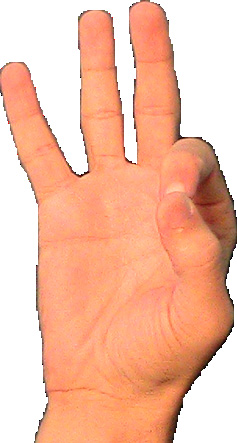
\includegraphics[scale=0.1]{images/09-01-1.jpg}&
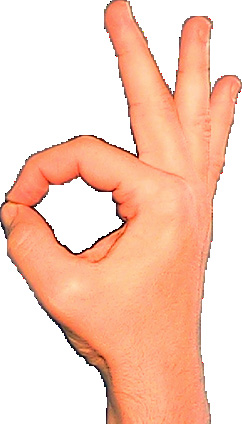
\includegraphics[scale=0.1]{images/09-01-2.jpg}&
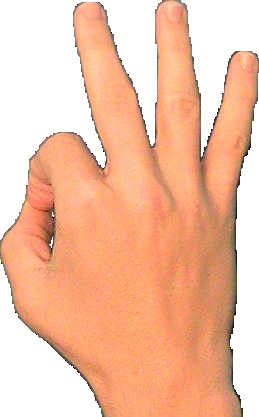
\includegraphics[scale=0.1]{images/09-01-3.jpg}&
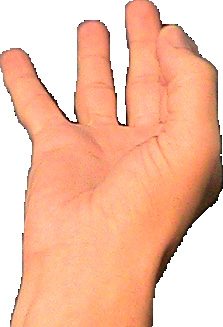
\includegraphics[scale=0.1]{images/09-01-4.jpg}&
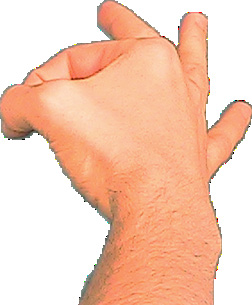
\includegraphics[scale=0.1]{images/09-01-5.jpg}&
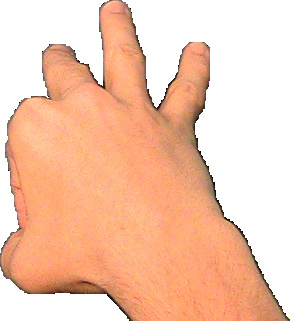
\includegraphics[scale=0.1]{images/09-01-6.jpg}\\
\textbf{Left}&
B509x515S18708491x486&
B509x515S18718491x486&
B509x515S18728491x486&
B509x515S18738491x486&
B509x515S18748491x486&
B509x515S18758491x486\\
\end{tabular}
\end{center}

\subsubsection{The Middle Ring Baby on Angle Handshape}

\begin{center}
\begin{tabular}{r*{6}{c}}
&\textbf{Fill 1}&\textbf{Fill 2}&\textbf{Fill 3}&\textbf{Fill 4}&\textbf{Fill 5}&\textbf{Fill 6}\\
\multirow{2}{*}{\textbf{Right}}&
B512x514S1d400489x486&
B512x514S1d410489x486&
B512x514S1d420489x486&
B512x514S1d430489x486&
B512x514S1d440489x486&
B512x514S1d450489x486\\
&
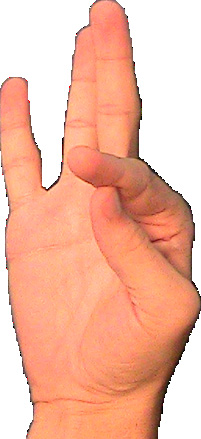
\includegraphics[scale=0.1]{images/09-02-1.jpg}&
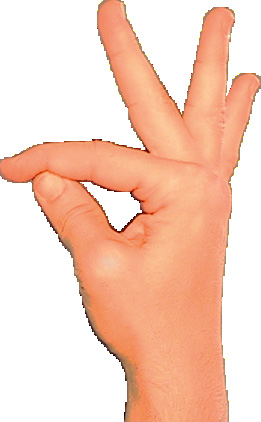
\includegraphics[scale=0.1]{images/09-02-2.jpg}&
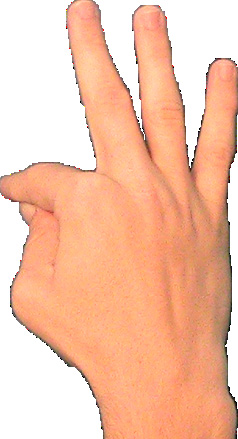
\includegraphics[scale=0.1]{images/09-02-3.jpg}&
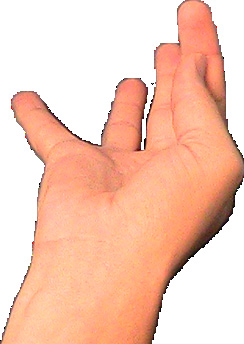
\includegraphics[scale=0.1]{images/09-02-4.jpg}&
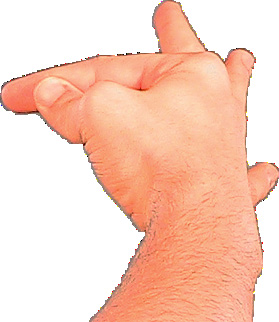
\includegraphics[scale=0.1]{images/09-02-5.jpg}&
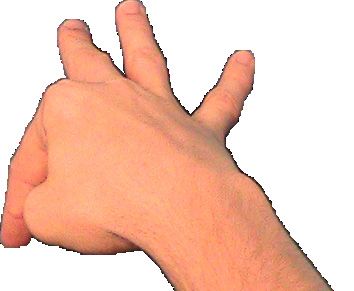
\includegraphics[scale=0.1]{images/09-02-6.jpg}\\
\textbf{Left}&
B512x514S1d408489x486&
B512x514S1d418489x486&
B512x514S1d428489x486&
B512x514S1d438489x486&
B512x514S1d448489x486&
B512x514S1d458489x486\\
\end{tabular}
\end{center}

\subsubsection{The Index Thumb Side Handshape}

\begin{center}
\begin{tabular}{r*{6}{c}}
&\textbf{Fill 1}&\textbf{Fill 2}&\textbf{Fill 3}&\textbf{Fill 4}&\textbf{Fill 5}&\textbf{Fill 6}\\
\multirow{2}{*}{\textbf{Right}}&
B511x515S1de00489x485&
B511x515S1de10489x485&
B511x515S1de20489x485&
B511x515S1de30489x485&
B511x515S1de40489x485&
B511x515S1de50489x485\\
&
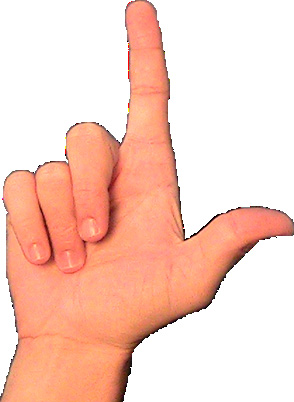
\includegraphics[scale=0.1]{images/09-03-1.jpg}&
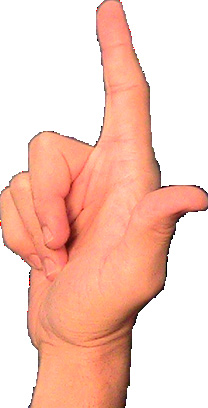
\includegraphics[scale=0.1]{images/09-03-2.jpg}&
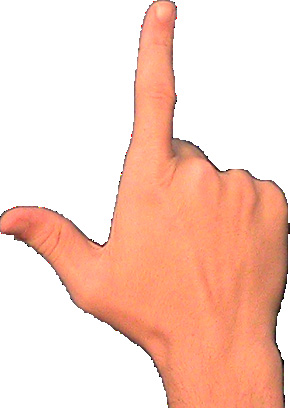
\includegraphics[scale=0.1]{images/09-03-3.jpg}&
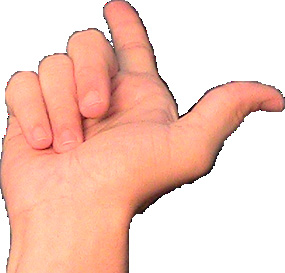
\includegraphics[scale=0.1]{images/09-03-4.jpg}&
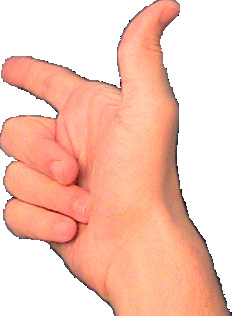
\includegraphics[scale=0.1]{images/09-03-5.jpg}&
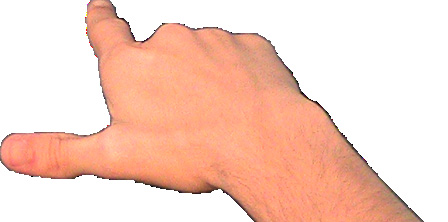
\includegraphics[scale=0.1]{images/09-03-6.jpg}\\
\textbf{Left}&
B511x515S1de08489x485&
B511x515S1de18489x485&
B511x515S1de28489x485&
B511x515S1de38489x485&
B511x515S1de48489x485&
B511x515S1de58489x485\\
\end{tabular}
\end{center}

\subsubsection{The Index Thumb Side, Thumb Bent Handshape}

\begin{center}
\begin{tabular}{r*{6}{c}}
&\textbf{Fill 1}&\textbf{Fill 2}&\textbf{Fill 3}&\textbf{Fill 4}&\textbf{Fill 5}&\textbf{Fill 6}\\
\multirow{2}{*}{\textbf{Right}}&
B512x515S1e000489x485&
B512x515S1e010489x485&
B512x515S1e020489x485&
B512x515S1e030489x485&
B512x515S1e040489x485&
B512x515S1e050489x485\\
&
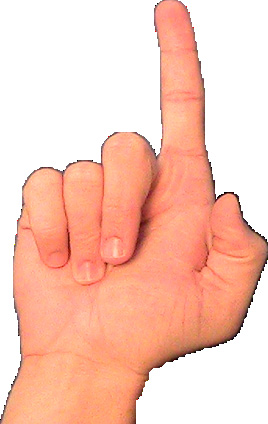
\includegraphics[scale=0.1]{images/09-04-1.jpg}&
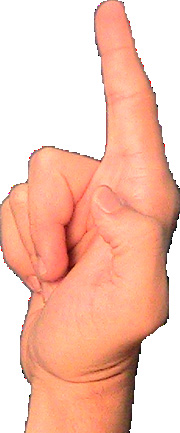
\includegraphics[scale=0.1]{images/09-04-2.jpg}&
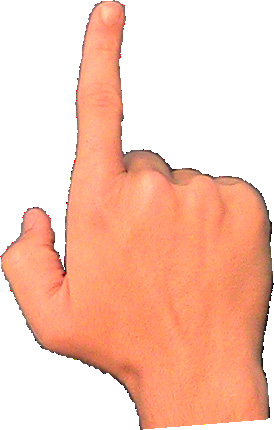
\includegraphics[scale=0.1]{images/09-04-3.jpg}&
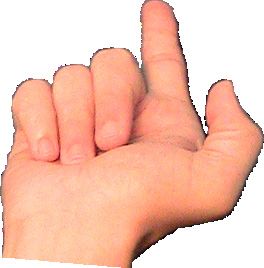
\includegraphics[scale=0.1]{images/09-04-4.jpg}&
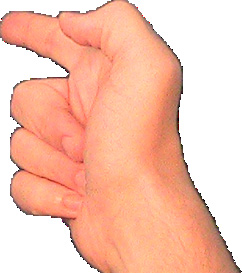
\includegraphics[scale=0.1]{images/09-04-5.jpg}&
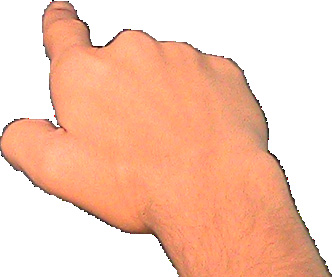
\includegraphics[scale=0.1]{images/09-04-6.jpg}\\
\textbf{Left}&
B512x515S1e008489x485&
B512x515S1e018489x485&
B512x515S1e028489x485&
B512x515S1e038489x485&
B512x515S1e048489x485&
B512x515S1e058489x485\\
\end{tabular}
\end{center}

\subsubsection{The Index Thumb Side, Index Bent Handshape}

\begin{center}
\begin{tabular}{r*{6}{c}}
&\textbf{Fill 1}&\textbf{Fill 2}&\textbf{Fill 3}&\textbf{Fill 4}&\textbf{Fill 5}&\textbf{Fill 6}\\
\multirow{2}{*}{\textbf{Right}}&
B512x513S1e100488x487&
B512x513S1e110488x487&
B512x513S1e120488x487&
B512x513S1e130488x487&
B512x513S1e140488x487&
B512x513S1e150488x487\\
&
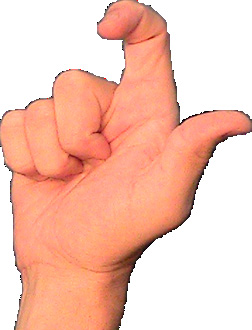
\includegraphics[scale=0.1]{images/09-05-1.jpg}&
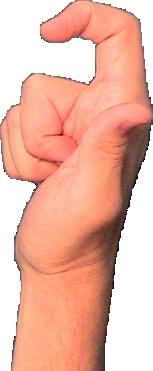
\includegraphics[scale=0.1]{images/09-05-2.jpg}&
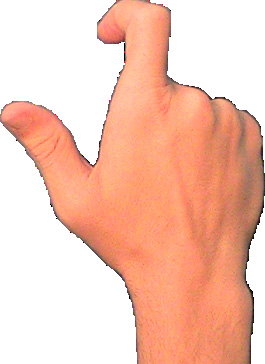
\includegraphics[scale=0.1]{images/09-05-3.jpg}&
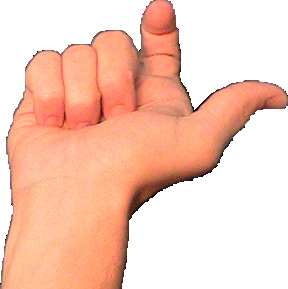
\includegraphics[scale=0.1]{images/09-05-4.jpg}&
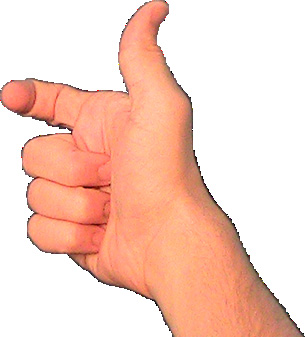
\includegraphics[scale=0.1]{images/09-05-5.jpg}&
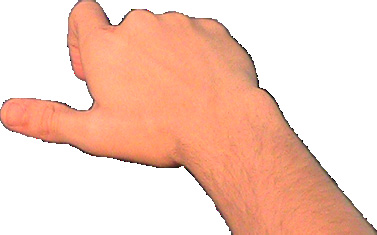
\includegraphics[scale=0.1]{images/09-05-6.jpg}\\
\textbf{Left}&
B512x513S1e108488x487&
B512x513S1e118488x487&
B512x513S1e128488x487&
B512x513S1e138488x487&
B512x513S1e148488x487&
B512x513S1e158488x487\\
\end{tabular}
\end{center}

\subsubsection{The Index Thumb Hook Handshape}

\begin{center}
\begin{tabular}{r*{6}{c}}
&\textbf{Fill 1}&\textbf{Fill 2}&\textbf{Fill 3}&\textbf{Fill 4}&\textbf{Fill 5}&\textbf{Fill 6}\\
\multirow{2}{*}{\textbf{Right}}&
B512x512S1e600489x488&
B512x512S1e610489x488&
B512x512S1e620489x488&
B512x512S1e630489x488&
B512x512S1e640489x488&
B512x512S1e650489x488\\
&
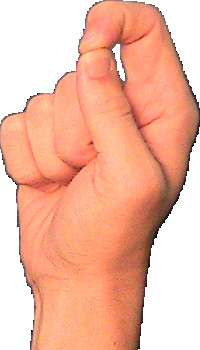
\includegraphics[scale=0.1]{images/09-06-1.jpg}&
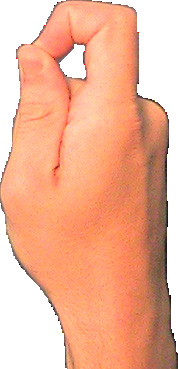
\includegraphics[scale=0.1]{images/09-06-2.jpg}&
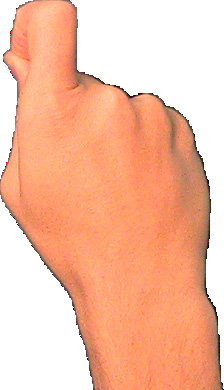
\includegraphics[scale=0.1]{images/09-06-3.jpg}&
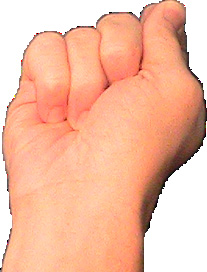
\includegraphics[scale=0.1]{images/09-06-4.jpg}&
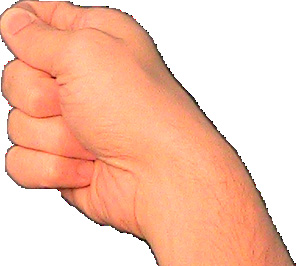
\includegraphics[scale=0.1]{images/09-06-5.jpg}&
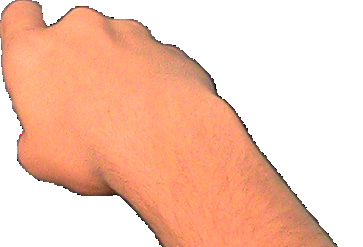
\includegraphics[scale=0.1]{images/09-06-6.jpg}\\
\textbf{Left}&
B512x512S1e608489x488&
B512x512S1e618489x488&
B512x512S1e628489x488&
B512x512S1e638489x488&
B512x512S1e648489x488&
B512x512S1e658489x488\\
\end{tabular}
\end{center}

\subsubsection{The Index Thumb Curve, Thumb Under Handshape}

\begin{center}
\begin{tabular}{r*{6}{c}}
&\textbf{Fill 1}&\textbf{Fill 2}&\textbf{Fill 3}&\textbf{Fill 4}&\textbf{Fill 5}&\textbf{Fill 6}\\
\multirow{2}{*}{\textbf{Right}}&
B512x511S1ea00489x490&
B512x511S1ea10489x490&
B512x511S1ea20489x490&
B512x511S1ea30489x490&
B512x511S1ea40489x490&
B512x511S1ea50489x490\\
&
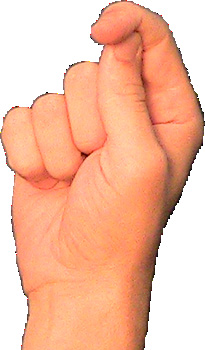
\includegraphics[scale=0.1]{images/09-07-1.jpg}&
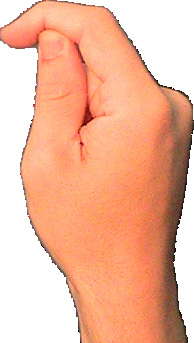
\includegraphics[scale=0.1]{images/09-07-2.jpg}&
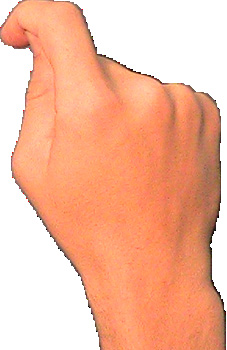
\includegraphics[scale=0.1]{images/09-07-3.jpg}&
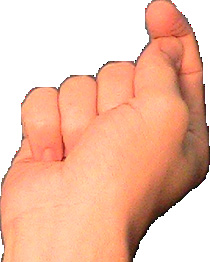
\includegraphics[scale=0.1]{images/09-07-4.jpg}&
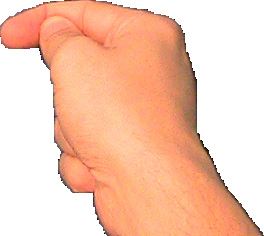
\includegraphics[scale=0.1]{images/09-07-5.jpg}&
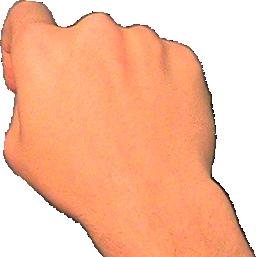
\includegraphics[scale=0.1]{images/09-07-6.jpg}\\
\textbf{Left}&
B512x511S1ea08489x490&
B512x511S1ea18489x490&
B512x511S1ea28489x490&
B512x511S1ea38489x490&
B512x511S1ea48489x490&
B512x511S1ea58489x490\\
\end{tabular}
\end{center}

\subsection{Vocabulary}

\begin{glossary}

\textbf{accident}\\
AS19a00S20500S30004M525x536S30004482x483S19a00486x516S20500515x510

\textbf{almost}\\
AS15a31S15a37S21100S26507M522x521S15a31478x487S15a37484x479S26507509x495S21100496x507

\textbf{article}\\
AS15a37S16c10S22b05M534x528S15a37467x473S16c10490x482S22b05510x504

\textbf{black board}\\
AS10051S10059S20500S27a02S27a1aS20500M535x545S10059465x470S10051502x469S20500493x455S20500501x534S27a1a474x500S27a02507x500

\textbf{campus}\\
AS10011S20500S2ff00S15a2fS15a37S22f04M539x572S20500502x518S10011518x499S2ff00482x483S15a37489x549S15a2f490x548S22f04488x531

\textbf{close captioned}\\
AS1ce40S1ce48S20500S20500S26a06S26a12S2fb04M525x533S1ce40503x467S1ce48475x467S26a06504x504S26a12484x503S20500496x504S20500496x515S2fb04494x527

\textbf{college}\\
AS15a51S15a07S28809S20e00M514x535S20e00492x490S28809494x465S15a07487x510S15a51488x512

\textbf{column}\\
AS15a37S16c10S22b05M534x528S15a37467x473S16c10490x482S22b05510x504

\textbf{deaf schoolL}\\
AS10011S20500S2ff00S15a2fS15a37S22f04M539x572S20500502x518S10011518x499S2ff00482x483S15a37489x549S15a2f490x548S22f04488x531

\textbf{easy}\\
AS15d02S15d0aS20e00S22f00M522x524S22f00487x477S20e00493x493S15d0a479x505S15d02495x500

\textbf{exam}\\
AS10620S10628S21600S21600S22c04S22c14S2fb04M528x542S10620507x470S10628475x470S22c04511x499S22c14473x500S21600507x458S21600488x458S2fb04494x536

\textbf{false}\\
AS10011S26602S20e00S33200M529x538S33200482x483S10011508x504S20e00492x526S26602457x518

\textbf{flash lights}\\
AS30000S18511S22100S21b00S22104S21600M555x518S30000482x483S18511522x455S21b00531x486S22100529x476S22104543x477S21600545x487

\textbf{graduate}\\
AS1f040S14c3aS2970cS20500M532x535S20500474x487S1f040483x466S14c3a469x511S2970c513x485

\textbf{hard}\\
AS11002S1100aS20e00S23110S23100S2fb04M538x529S11002511x472S1100a468x477S23100512x501S23110463x502S20e00495x505S2fb04493x523

\textbf{hard of hearing}\\
AS11541S22f04S26606M526x523S11541474x477S22f04492x509S26606496x494

\textbf{high school}\\
M525x508S11502475x493S20320510x493

\textbf{interpreter}\\
AS1ce10S1ce1fS20500S2c400S2f900M537x532S1ce10489x491S1ce1f463x497S20500484x521S2c400497x468S2f900518x495

\textbf{list}\\
AS14402S1440aS22b04M518x537S14402485x487S1440a482x464S22b04502x507

\textbf{mistake}\\
AS19a00S20500S30004M525x536S30004482x483S19a00486x516S20500515x510

\textbf{note}\\
AS18511S15a38S20500S20500S20500S28802S28802S28802M534x529S15a38474x486S18511480x485S28802509x471S28802512x502S28802511x487S20500493x518S20500480x518S20500467x518

\textbf{perimeter}\\
AS10051S10059S20500S27a02S27a1aS20500M535x545S10059465x470S10051502x469S20500493x455S20500501x534S27a1a474x500S27a02507x500

\textbf{quiz}\\
AS10620S10628S21600S21600S22c04S22c14S2fb04M528x542S10620507x470S10628475x470S22c04511x499S22c14473x500S21600507x458S21600488x458S2fb04494x536

\textbf{research}\\
AS10050S15a3aS20e00S26a06M521x527S15a3a480x474S10050489x496S20e00497x488S26a06507x500

\textbf{sign}\\
AS10051S10059S20500S27a02S27a1aS20500M535x545S10059465x470S10051502x469S20500493x455S20500501x534S27a1a474x500S27a02507x500

\textbf{square}\\
AS10051S10059S20500S27a02S27a1aS20500M535x545S10059465x470S10051502x469S20500493x455S20500501x534S27a1a474x500S27a02507x500

\textbf{test}\\
AS10620S10628S21600S21600S22c04S22c14S2fb04M528x542S10620507x470S10628475x470S22c04511x499S22c14473x500S21600507x458S21600488x458S2fb04494x536

\textbf{university}\\
AS15a51S15a07S28809S20e00M514x535S20e00492x490S28809494x465S15a07487x510S15a51488x512

\textbf{write (horizontally)}\\
AS1eb20S15a39S26507M527x518S15a39474x483S1eb20490x499S26507514x485

\textbf{write (vertically / SignWriting)}\\
AS1eb10S15a18S22b04M519x527S15a18482x475S1eb10495x474S22b04503x497

\textbf{wrong}\\
AS19a00S20500S30004M525x536S30004482x483S19a00486x516S20500515x510

\end{glossary}

\subsection{Practice Sheet 13.A}

\begin{multicols}{5}
\begin{center}

M508x515S10000493x485 % 1
M536x504S38800464x496 % .
M521x527S15a3a480x474S10050489x496S20e00497x488S26a06507x500 % research
M534x528S15a37467x473S16c10490x482S22b05510x504 % article
M537x504S38700463x496 % ,
M518x518S30a00482x483 % y/n
M510x523S10040495x493S26500491x478 % you
M516x540S1bb02488x461S14c02484x517S20e00499x502S26500499x483 % like
M524x525S10e41499x481S15a07477x475S22b03479x501 % read
M536x507S38900464x493 % ?
\vfil
\columnbreak

M508x515S10e00493x485 % 2
M536x504S38800464x496 % .
M518x518S30a00482x483 % y/n
M507x523S15a28494x496S26500493x477 % your
M508x510S1fb20493x491 % t
M508x515S10e20493x485 % v
M525x533S1ce40503x467S1ce48475x467S26a06504x504S26a12484x503S20500496x504S20500496x515S2fb04494x527 % close captioned
M536x507S38900464x493 % ?
\vfil
\columnbreak

M512x515S11e00489x485 % 3
M536x504S38800464x496 % .
M518x518S30a00482x483 % y/n
M507x523S15a28494x496S26500493x477 % your
M518x518S2ff00482x483S20500495x469S14c10468x453 % father
M514x535S20e00492x490S28809494x465S15a07487x510S15a51488x512 % college
M536x507S38900464x493 % ?
\vfil
\columnbreak

M511x516S14400489x485 % 4
M536x504S38800464x496 % .
M518x518S30a00482x483 % y/n
M510x523S10040495x493S26500491x478 % you
M580x518S31410482x483S1dc21511x483S1f410551x489S26506541x494 % gallaudet
M510x523S10040495x493S26500491x478 % you
M536x507S38900464x493 % ?
\vfil
\columnbreak

M512x516S14c00489x485 % 5
M536x504S38800464x496 % .
M518x518S30a00482x483 % y/n
M534x543S14c30507x457S14c38469x458S15030508x512S15038467x511S26524493x493 % want
M521x539S15a07494x489S15a21498x490S2df04498x518S2df14497x462S21100479x487 % become
M537x532S1ce10489x491S1ce1f463x497S20500484x521S2c400497x468S2f900518x495 % interpreter
M510x523S10040495x493S26500491x478 % you
M536x507S38900464x493 % ?
\vfil

\end{center}
\end{multicols}

\subsection{Practice Sheet 13.B}

\begin{multicols}{5}
\begin{center}

M509x515S18720491x486 % 6
M536x504S38800464x496 % .
M518x518S30c00482x483 % \?
L544x531S20500509x515S10011523x501S20500520x488S2ff00482x483 % deaf
R533x549S2ff00482x483S2ea08491x524S10012503x508 % hearing
M510x523S10040495x493S26500491x478 % you
M536x507S38900464x493 % ?
\vfil
\columnbreak

M511x514S1a520490x486 % 7
M536x504S38800464x496 % .
M518x518S30a00482x483 % y/n
M510x523S10040495x493S26500491x478 % you
M539x519S2ff00482x483S10011518x489S20500510x474 % think
M526x523S11541474x477S22f04492x509S26606496x494 % hard of hearing
M514x524S10620486x476S23004489x506 % should
M528x528S22b03504x472S17107478x502S16d21472x508 % marry
M544x531S20500509x515S10011523x501S20500520x488S2ff00482x483 % deaf
M508x508S17620492x492 % o
M508x515S11a20493x485 % r
M533x549S2ff00482x483S2ea08491x524S10012503x508 % hearing
M536x507S38900464x493 % ?
\vfil
\columnbreak

M511x514S1bb20490x486 % 8
M536x504S38800464x496 % .
M525x508S11502475x493S20320510x493 % high school
M537x504S38700463x496 % ,
M518x518S30c00482x483 % \?
M510x523S10040495x493S26500491x478 % you
M532x535S20500474x487S1f040483x466S14c3a469x511S2970c513x485 % graduate
M536x522S10019464x492S10012487x492S2e708521x486S20500476x478 % when
M536x507S38900464x493 % ?
\vfil
\columnbreak

M511x515S1ce20489x485 % 9
M536x504S38800464x496 % .
M518x518S30a00482x483 % y/n
M510x523S10040495x493S26500491x478 % you
M539x519S2ff00482x483S10011518x489S20500510x474 % think
M509x520S10004492x480S22a04496x505 % this
M527x528S16d10509x508S16d18473x508S2df06507x479S2df1e473x480S2fb00493x473 % class
M538x529S11002511x472S1100a468x477S23100512x501S23110463x502S20e00495x505S2fb04493x523 % hard
M536x507S38900464x493 % ?
\vfil
\columnbreak

M513x528S2a538494x472S1f540488x504 % 10
M536x504S38800464x496 % .
M544x531S20500509x515S10011523x501S20500520x488S2ff00482x483 % deaf
M514x535S20e00492x490S28809494x465S15a07487x510S15a51488x512 % college
M543x638S15a37480x556S14c51501x539S22c00520x503S20500512x467S18510518x482S2ff00482x483S20500487x562S15a40509x591S15a48482x590S22a24494x623 % student
M528x521S15a39473x479S10041482x491S20e00497x490S2ea00513x483 % sometimes
M526x524S20308504x509S11500511x477S20e00496x493S22f02477x486S37706474x516 % use
M534x529S15a38474x486S18511480x485S28802509x471S28802512x502S28802511x487S20500493x518S20500480x518S20500467x518 % note
M532x534S14c50508x503S20358472x466S20350512x466S22a00513x484S14c58468x503S22a10473x484S2fb00492x485 % take
M537x504S38700463x496 % ,
M574x535S22a05540x506S15d11520x488S19a37551x508S30c00482x483 % why?
M536x507S38900464x493 % ?
\vfil

\end{center}
\end{multicols}

\subsection{Practice Sheet 13.C}

\begin{multicols}{5}
\begin{center}

M512x520S10000489x490S21d00494x480 % 11
M536x504S38800464x496 % .
M518x564S26500492x549S1e301486x518S2ff00482x483 % observe
M542x523S10058459x493S14c10482x477S20500476x501S2a502509x490 % movie
M537x504S38700463x496 % ,
M518x518S30a00482x483 % y/n
M510x523S10040495x493S26500491x478 % you
M516x540S1bb02488x461S14c02484x517S20e00499x502S26500499x483 % like
M525x533S1ce40503x467S1ce48475x467S26a06504x504S26a12484x503S20500496x504S20500496x515S2fb04494x527 % close capiton
M536x507S38900464x493 % ?
\vfil
\columnbreak

M509x521S10e00491x491S21d00491x480 % 12
M536x504S38800464x496 % .
M534x541S33b00482x483S10010487x511S26500520x497 % true
M529x538S33200482x483S10011508x504S20e00492x526S26602457x518 % false
M528x542S10620507x470S10628475x470S22c04511x499S22c14473x500S21600507x458S21600488x458S2fb04494x536 % test
M537x504S38700463x496 % ,
M518x518S30a00482x483 % y/n
M510x523S10040495x493S26500491x478 % you
M516x540S1bb02488x461S14c02484x517S20e00499x502S26500499x483 % like
M536x507S38900464x493 % ?
\vfil
\columnbreak

M513x519S22114487x481S12d00489x489 % 13
M536x504S38800464x496 % .
M521x527S15a3a480x474S10050489x496S20e00497x488S26a06507x500 % research
M528x530S15d3a497x496S15d51505x507S20e00492x481S26a01473x471S20e00483x491 % paper
M537x504S38700463x496 % ,
M518x518S30a00482x483 % y/n
M510x523S10040495x493S26500491x478 % you
M516x540S1bb02488x461S14c02484x517S20e00499x502S26500499x483 % like
M527x518S15a39474x483S1eb20490x499S26507514x485 % write
M536x507S38900464x493 % ?
\vfil
\columnbreak

M513x515S14700493x493S22114487x486 % 14
M536x504S38800464x496 % .
M546x575S2ff00482x483S18510521x490S18518452x493S26500525x468S26510458x469S15a40507x524S15a48481x525S22a24493x560 % teacher
M555x518S30000482x483S18511522x455S21b00531x486S22100529x476S22104543x477S21600545x487 % lights flash
M537x504S38700463x496 % ,
M574x535S22a05540x506S15d11520x488S19a37551x508S30c00482x483 % why?
M536x507S38900464x493 % ?
\vfil
\columnbreak

M513x518S22114487x483S15d00494x491 % 15
M536x504S38800464x496 % .
M537x532S1ce10489x491S1ce1f463x497S20500484x521S2c400497x468S2f900518x495 % interpreter
M518x537S14402485x487S1440a482x464S22b04502x507 % list
M537x504S38700463x496 % ,
M518x518S30a00482x483 % y/n
M510x523S10040495x493S26500491x478 % you
M532x518S18049468x483S18041507x483S20500486x507S20500504x507 % have
M536x507S38900464x493 % ?
\vfil

\end{center}
\end{multicols}

\subsection{Practice Sheet 13.D}

\begin{multicols}{5}
\begin{center}

M520x522S18700502x492S2e00e480x479 % 16
M536x504S38800464x496 % .
M535x545S10059465x470S10051502x469S20500493x455S20500501x534S27a1a474x500S27a02507x500 % square
M537x504S38700463x496 % ,
M510x523S10040495x493S26500491x478 % you
M539x519S2ff00482x483S10011518x489S20500510x474 % think
M515x519S10047485x498S26507501x481 % 3rd person
M546x575S2ff00482x483S18510521x490S18518452x493S26500525x468S26510458x469S15a40507x524S15a48481x525S22a24493x560 % teacher
M514x524S10620486x476S23004489x506 % should
M527x518S15a39474x483S1eb20490x499S26507514x485 % write
M526x517S18510501x502S18518475x502S20500495x484 % more
M536x507S38900464x493 % ?
\vfil
\columnbreak

M522x522S1a500501x494S2e00e478x478 % 17
M536x504S38800464x496 % .
M518x518S30c00482x483 % \?
M547x530S36d00479x487S15d00528x470S26604527x500 % past
M528x542S10620507x470S10628475x470S22c04511x499S22c14473x500S21600507x458S21600488x458S2fb04494x536 % test
M509x520S10004492x480S22a04496x505 % this
M527x528S16d10509x508S16d18473x508S2df06507x479S2df1e473x480S2fb00493x473 % class
M510x523S10040495x493S26500491x478 % you
M525x536S30004482x483S19a00486x516S20500515x510 % wrong
M526x535S22a20494x501S14c08474x465S14c00503x465S20338478x520S20330508x520 % how many
M536x507S38900464x493 % ?
\vfil
\columnbreak

M523x522S1bb00502x492S2e00e478x479 % 18
M536x504S38800464x496 % .
M514x535S20e00492x490S28809494x465S15a07487x510S15a51488x512 % college
M537x504S38700463x496 % ,
M518x518S30c00482x483 % \?
M510x523S10040495x493S26500491x478 % you
M532x535S20500474x487S1f040483x466S14c3a469x511S2970c513x485 % graduate
M536x522S10019464x492S10012487x492S2e708521x486S20500476x478 % when
M536x507S38900464x493 % ?
\vfil
\columnbreak

M524x522S1ce00502x490S2e00e477x479 % 19
M536x504S38800464x496 % .
M518x518S30a00482x483 % y/n
M510x523S10040495x493S26500491x478 % you
M539x519S2ff00482x483S10011518x489S20500510x474 % think
M509x520S10004492x480S22a04496x505 % this
M527x528S16d10509x508S16d18473x508S2df06507x479S2df1e473x480S2fb00493x473 % class
M522x524S22f00487x477S20e00493x493S15d0a479x505S15d02495x500 % easy
M536x507S38900464x493 % ?
\vfil
\columnbreak

M517x513S22114484x488S1f420488x498 % 20
M536x504S38800464x496 % .
M518x518S30a00482x483 % y/n
M539x572S20500502x518S10011518x499S2ff00482x483S15a37489x549S15a2f490x548S22f04488x531 % deaf school
M510x523S10040495x493S26500491x478 % you
M536x507S38900464x493 % ?
\vfil

\end{center}
\end{multicols}

\subsection{Story 13}

\begin{multicols}{5}
\begin{center}

M518x518S10043488x483S20500482x507 % me
M539x572S20500502x518S10011518x499S2ff00482x483S15a37489x549S15a2f490x548S22f04488x531 % deaf school
M508x508S17620492x492 % o
M515x508S1f000486x493 % g
M508x515S10110492x485 % d
M508x508S14a20493x493 % e
M511x513S11920490x487 % n
M537x504S38700463x496 % ,
M508x515S11520493x485 % u
M508x510S1fb20493x491 % t
M510x508S1f720490x493 % a
M515x508S11502485x493 % h
M537x504S38700463x496 % ,
M532x535S20500474x487S1f040483x466S14c3a469x511S2970c513x485 % graduate
M524x522S1ce00502x490S2e00e477x479 % 19
M522x516S14420500x485S1bb20478x488 % 84
M536x504S38800464x496 % .

M535x522S22f14466x501S22f04510x501S2fb04494x516S18215468x479S1821d508x479 % now
M514x535S20e00492x490S28809494x465S15a07487x510S15a51488x512 % college
M509x510S16d20492x490 % c
M508x508S20320493x493 % s
M508x515S11520493x485 % u
M511x513S11920490x487 % n
M536x504S38800464x496 % .

M518x518S10043488x483S20500482x507 % me
M516x540S1bb02488x461S14c02484x517S20e00499x502S26500499x483 % like
M514x535S20e00492x490S28809494x465S15a07487x510S15a51488x512 % college
M537x504S38700463x496 % ,
M526x521S10021496x500S10029475x500S26506507x480S26512475x480 % but
M538x529S11002511x472S1100a468x477S23100512x501S23110463x502S20e00495x505S2fb04493x523 % hard
M536x504S38800464x496 % .

M525x508S11502475x493S20320510x493 % high school
M522x524S22f00487x477S20e00493x493S15d0a479x505S15d02495x500 % easy
M536x504S38800464x496 % .

M535x522S22f14466x501S22f04510x501S2fb04494x516S18215468x479S1821d508x479 % now
M512x524S10620489x476S22e04495x506 % must
M524x525S10e41499x481S15a07477x475S22b03479x501 % read
M534x528S15a37467x473S16c10490x482S22b05510x504 % article
M536x504S38800464x496 % .

M527x518S15a39474x483S1eb20490x499S26507514x485 % write
M521x527S15a3a480x474S10050489x496S20e00497x488S26a06507x500 % reasearch
M528x530S15d3a497x496S15d51505x507S20e00492x481S26a01473x471S20e00483x491 % paper
M536x504S38800464x496 % .

M546x575S2ff00482x483S18510521x490S18518452x493S26500525x468S26510458x469S15a40507x524S15a48481x525S22a24493x560 % teacher
M535x545S10059465x470S10051502x469S20500493x455S20500501x534S27a1a474x500S27a02507x500 % square
M527x518S15a39474x483S1eb20490x499S26507514x485 % write
M512x524S10620489x476S22e04495x506 % must
M522x531S2b720489x469S18527503x504S1852f479x503 % put
M536x504S38800464x496 % .

M537x532S1ce10489x491S1ce1f463x497S20500484x521S2c400497x468S2f900518x495 % interpreter
M537x504S38700463x496 % ,
M512x524S10620489x476S22e04495x506 % must
M518x564S26500492x549S1e301486x518S2ff00482x483 % observe
M536x504S38800464x496 % .

M518x518S30c00482x483 % \?
M574x535S22a05540x506S15d11520x488S19a37551x508S30c00482x483 % why?

M528x542S10620507x470S10628475x470S22c04511x499S22c14473x500S21600507x458S21600488x458S2fb04494x536 % test
M538x529S11002511x472S1100a468x477S23100512x501S23110463x502S20e00495x505S2fb04493x523 % hard

\end{center}
\end{multicols}

\end{document}

